% Compare analytical, supervised learning, imitation learning and lead into reinforcement learning
% Say what is novel - 3D observations
\begin{frame}{Vision-Based Robotic Grasping of Diverse Objects}{}
    \begin{columns}%
        \begin{column}{0.5\textwidth}%
            \centering
            \hspace{-0.5cm}
            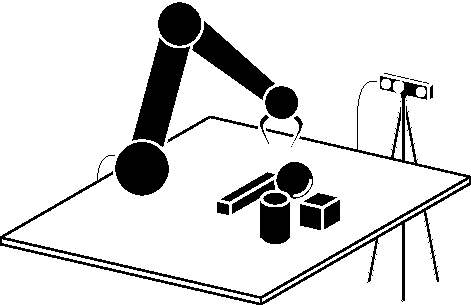
\includegraphics[height=4.75cm]{graphics/setup_sketch.pdf}
        \end{column}
        %
        \begin{column}{0.5\textwidth}%
            \centering
            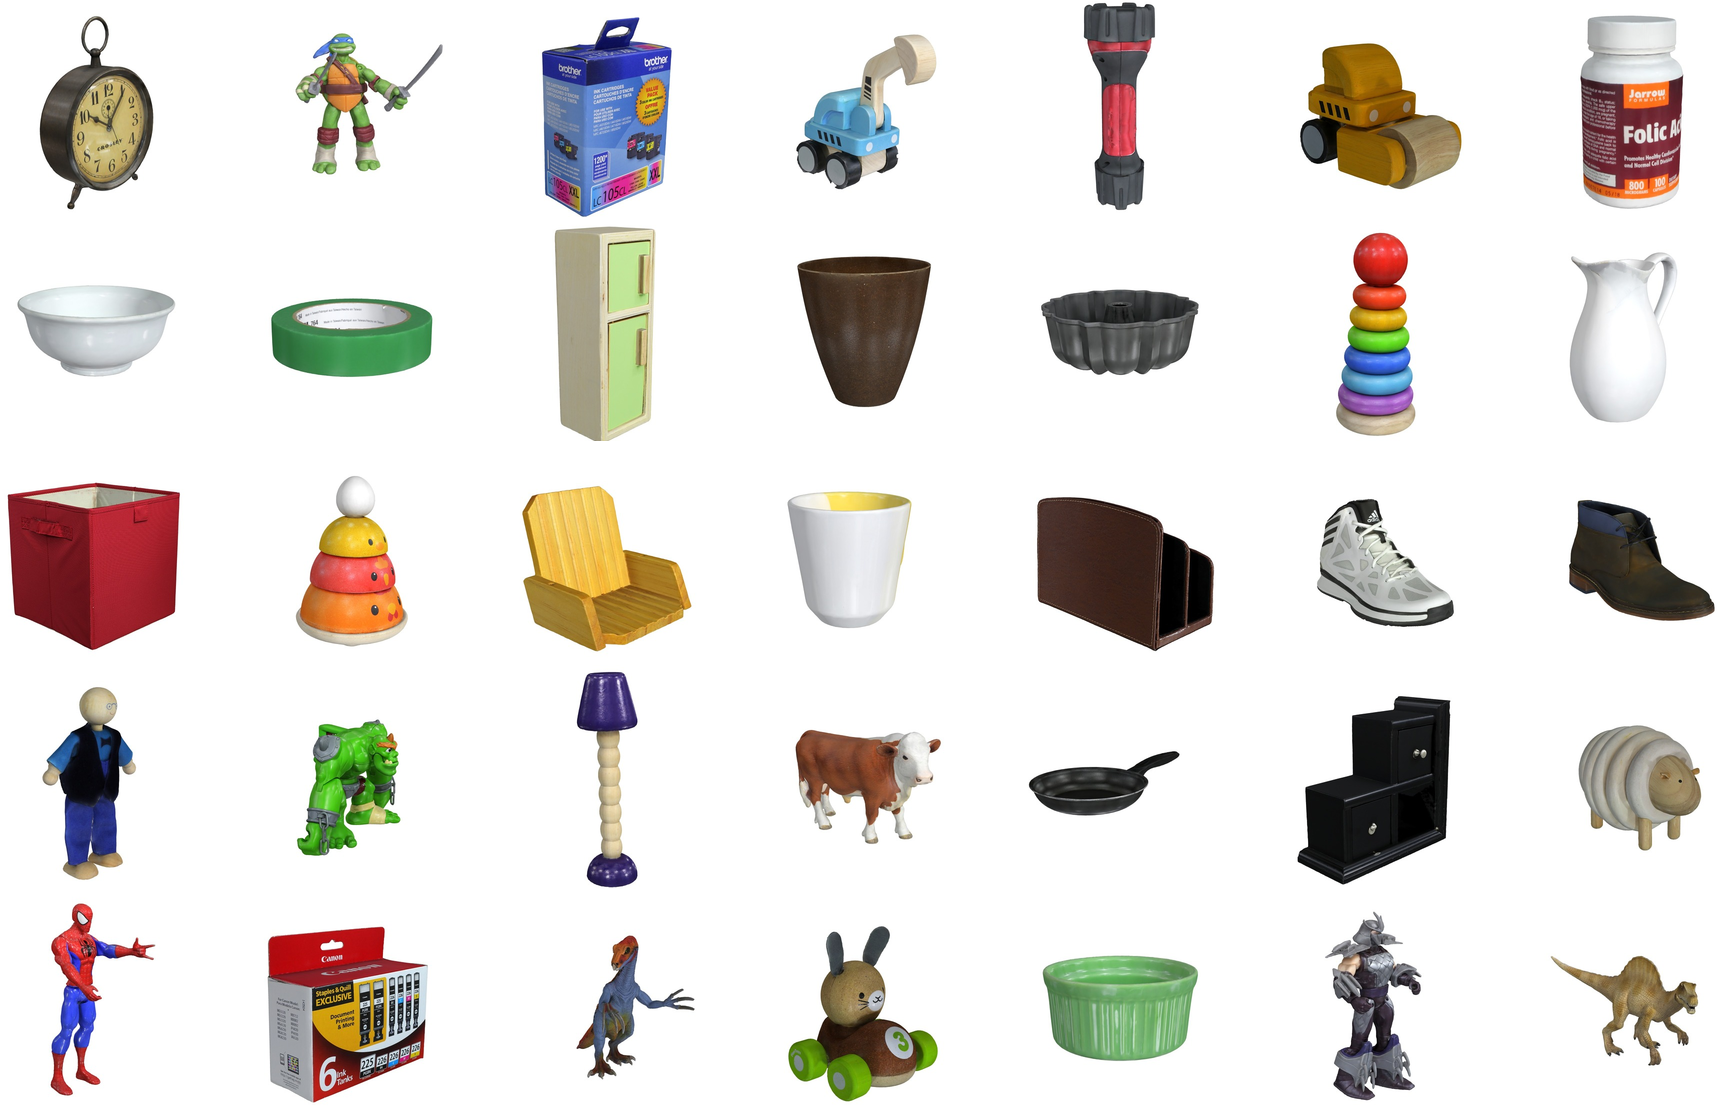
\includegraphics[height=4.75cm]{graphics/training_set.png}
        \end{column}
    \end{columns}
\end{frame}

\begin{frame}{Vision-Based Robotic Grasping of Diverse Objects}{Approach}
    \begin{columns}%
        \begin{column}{0.375\textwidth}%
            \begin{block}{Approaches}
                \begin{itemize}
                    \item Analytical
                    \item Empirical
                    \begin{itemize}
                        \item Supervised Learning
                        \item Imitation Learning
                        \item \only<1>{Reinforcement Learning}\only<2>{\textbf{Reinforcement Learning}}
                    \end{itemize}
                \end{itemize}
            \end{block}
        \end{column}
        %
        \begin{column}{0.625\textwidth}%
            \centering
            \onslide<2>{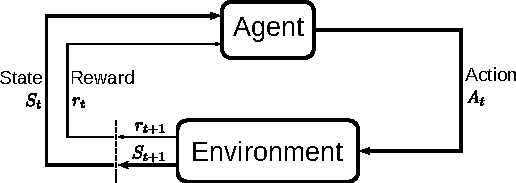
\includegraphics[width=\textwidth]{graphics/mdp_loop.pdf}}
        \end{column}
    \end{columns}
\end{frame}

% Task Definition, MDP formulation
\begin{frame}{Task Definition}{}
    \begin{columns}%
        \begin{column}{0.32\textwidth}%
            \begin{block}{Agent}
                \begin{itemize}
                    \item High-level controller
                    \item End-to-end policy
                \end{itemize}
            \end{block}
        \end{column}
        %
        \begin{column}{0.32\textwidth}%
            \begin{block}{Environment}
                \begin{itemize}
                    \item Objects
                    \item Robot
                    \begin{itemize}
                        \item Low-level controllers
                    \end{itemize}
                    \item Physics and visuals
                \end{itemize}
            \end{block}
        \end{column}
        %
        \begin{column}{0.35\textwidth}%
            \begin{block}{Episodic Task}
                \begin{itemize}
                    \item Success
                    \begin{itemize}
                        \item Lifting an object
                    \end{itemize}
                    \item Failure
                    \begin{itemize}
                        \item Pushing all objects away
                    \end{itemize}
                    \item Max 100 time steps
                    \begin{itemize}
                        \item \textasciitilde 40 s (simulation)
                    \end{itemize}
                \end{itemize}
            \end{block}
        \end{column}
    \end{columns}
\end{frame}

% Action space - say that Cartesian was selected and why. Why not full 3D space. Maybe also mention why relative motion is selected.
\begin{frame}{Action Space}{}
    \begin{columns}%
        \begin{column}{0.4\textwidth}%
            \begin{block}{Actions in Cartesian space}
                \begin{itemize}
                    \item Translational displacement
                    \begin{itemize}
                        \item \((d_{x},d_{y},d_{z})\)
                    \end{itemize}
                    \item Gripper rotation \(d_{\phi}\)
                    \item Gripper actions \(g\)
                    \begin{itemize}
                        \item Closing
                        \item Opening
                    \end{itemize}
                \end{itemize}
            \end{block}
        \end{column}
        %
        \begin{column}{0.6\textwidth}%
            \centering
            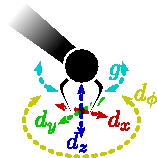
\includegraphics[height=6cm]{graphics/action_space.pdf}
        \end{column}
    \end{columns}
\end{frame}
